Wie im Kapitel \ref{chap:quantile} gezeigt wurde scheint sich die Abweichung des 99. Quantils des Niederschlags (und damit des Starkregens) bei allen Datensätzen nahezu identisch abzuzeichnen. Deshalb soll in diesem Kapitel wie es in \cite{biasMaraun} gemacht wurde, gezielt auf die Starkregenereignisse der unterschiedlichen Jahreszeiten eingegangen werden um die Evaluation der beiden Klimamodelle abzuschließen.
\section{Herangehensweise}\label{sec:Herangehensweise}
\begin{itemize}
\item Alle Datensätze werden auf die Jahreszeiten aufgeteilt:
	\subitem Frühling: 20.März - 20.Juni
	\subitem Sommer: 20.Juni - 22. September
	\subitem Herbst: 22.September - 21. Dezember
	\subitem Winter: 21. Dezember - 20. März
\item Von diesen neu aufgeteilten Datensätzen werden die 99. Quantile berechnet
\item Diese Quantile werden mit den Beobachtungsdaten verglichen.
\end{itemize}

\section{Differenzen im den Jahreszeiten}
Es wurde wie im Unterkapitel \ref{sec:Herangehensweise} erklärt, die Daten zunächst auf die Jahreszeiten aufgeteilt und dann daraus (über alle zehn Jahre) die maximalen Niederschläge herausgefiltert - über die Berechnung des 99.Quantils. Danach wurde wie schon in den Kapiteln zuvor beschrieben von den Modelldaten die Beobachtungsdaten abgezogen-das heißt wenn die Differenz negativ ist wurde zu wenig Niederschlagsmenge modelliert, und vice versa.\\
Aus diesen Abweichungen wurden die Boxplots in Abb.\ref{fig:seasons_boxplots} erstellt: Alle Abweichungen scheinen sich in einem relativ guten Rahmen aufzuhalten. Nur der Evaluation-Datensatz aus ALP-3 scheint enorme Ausreißer zu haben. Dies ist wiederum auf das Gebiet im Süden Kroatiens zurückzuführen wie in der Abbildung \ref{fig:seasons_dif} zu erkennen ist. In der Tabelle \ref{tab:season_bias} wurden die schlechtesten Performance nach der Jahreszeit der Datensätze eingetragen. Da hier nur drei von zwei Datensätze auftauchten wurde noch eine zweite Tabelle angelegt, die die schlechteste Jahreszeit für jeden Datensatzes darstellt. Diese ist in Tabelle \ref{tab:season_dataset} untergebracht. Die Einträge der Tabelle\ref{tab:season_dataset} und der Tabelle\ref{tab:season_bias} wurden dann verwendet um über die Datensätze der Folgenden näheren Betrachtungen zu entscheiden:
\begin{itemize}
	\item Für den Datensatz Historical EUR-11: Frühling
	\item Für den Datensatz Evaluation EUR-11: Sommer
	\item Für den Datensatz Historical ALP-3: Sommer
	\item Für den Datensatz Evaluation ALP-3: Frühling
\end{itemize}
Da dadurch die Datensätze für das selbe Phänomen untereinander verglichen werden konnten. 
\begin{table}[h]
	\begin{tabularx}{\textwidth}{|X|X|X|X|}
		\hline
		\textbf{Frühling} & \textbf{Sommer}& \textbf{Herbst} & \textbf{Winter}\\
		\hline
		\textbf{Evaluation ALP-3}  & \textbf{Historical ALP-3}  & \textbf{Evaluation EUR-11} & \textbf{Historical ALP-3} \\
		Bias:$7.01032\frac{mm}{Tag}$& Bias:$6.68616\frac{mm}{Tag}$ & Bias: $-4.28896\frac{mm}{Tag}$ & Bias:$8.33802\frac{mm}{Tag}$\\
		\hline
	\end{tabularx}
	\caption{Schlechteste Performance nach Extremniederschlägen in den Jahreszeiten gemessen am Bias}
	\label{tab:season_bias}
\end{table}
\begin{table}[h]
	\begin{tabularx}{\textwidth}{|X|X|X|X|}
		\hline
		\textbf{Historical EUR-11} & \textbf{Evaluation EUR-11}& \textbf{Historical ALP-3} & \textbf{Evaluation ALP-3}\\
		\hline
		\textbf{Frühling}  & \textbf{Sommer}  & \textbf{Winter} & \textbf{Frühling} \\
		Bias:$5.36773\frac{mm}{Tag}$& Bias:$5.33069\frac{mm}{Tag}$ & Bias:$8.33802\frac{mm}{Tag}$ & Bias:$7.01032\frac{mm}{Tag}$\\
		\hline
	\end{tabularx}
	\caption{Schlechteste Performance der einzelnen Datensätze nach Extremniederschlägen in den Jahreszeiten gemessen am Bias}
	\label{tab:season_dataset}
\end{table}
\begin{figure}
	\begin{subfigure}{0.49\textwidth}
		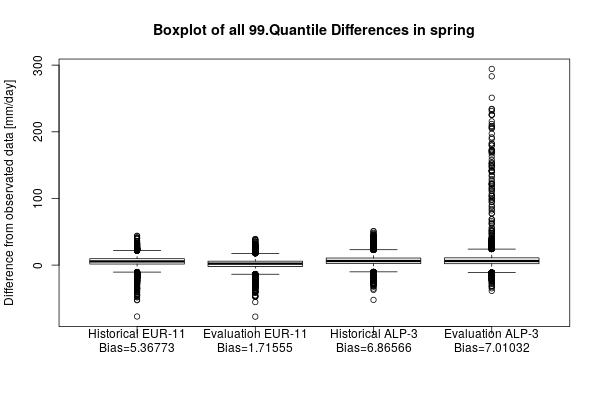
\includegraphics[width=\textwidth]{quantile_season/boxplot_spring.jpg}
		\caption{Frühling}
	\end{subfigure}
	\begin{subfigure}{0.49\textwidth}
		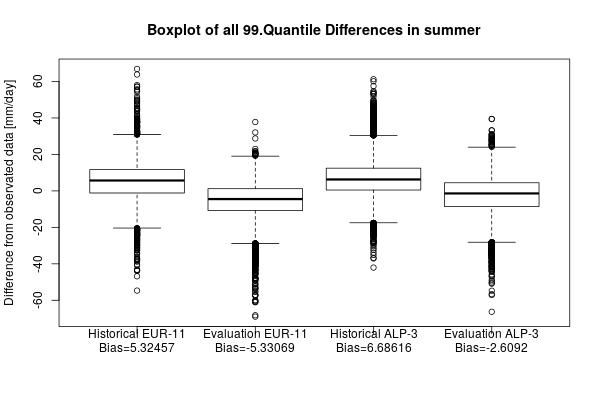
\includegraphics[width=\textwidth]{quantile_season/boxplot_summer.jpg}
		\caption{Sommer}
	\end{subfigure}
	\begin{subfigure}{0.49\textwidth}
		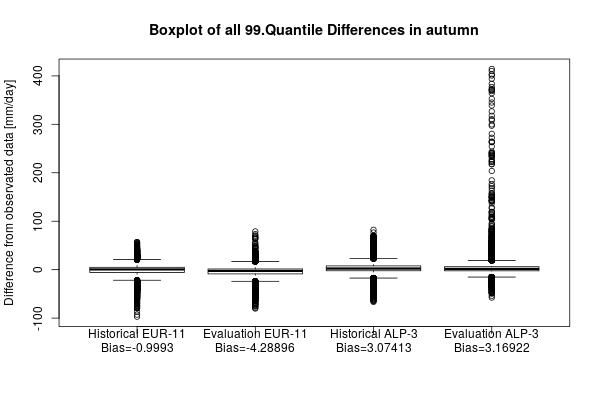
\includegraphics[width=\textwidth]{quantile_season/boxplot_autumn.jpg}
		\caption{Herbst}
	\end{subfigure}
	\begin{subfigure}{0.49\textwidth}
		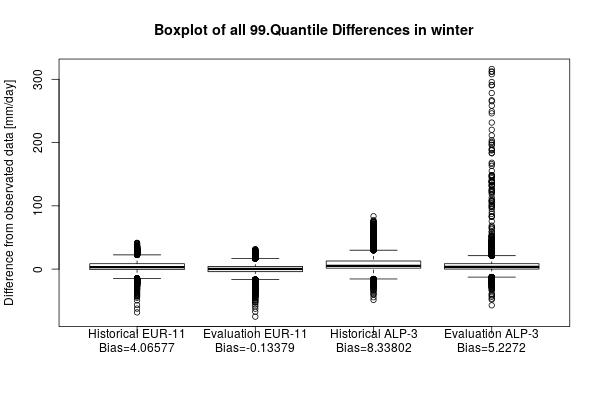
\includegraphics[width=\textwidth]{quantile_season/boxplot_winter.jpg}
		\caption{Winter}
	\end{subfigure}
	\caption{Boxplots der Starkniederschläge in den verschiedenen Jahreszeiten}
	\label{fig:seasons_boxplots}
\end{figure}
\begin{figure}
	\begin{subfigure}{0.49\textwidth}
		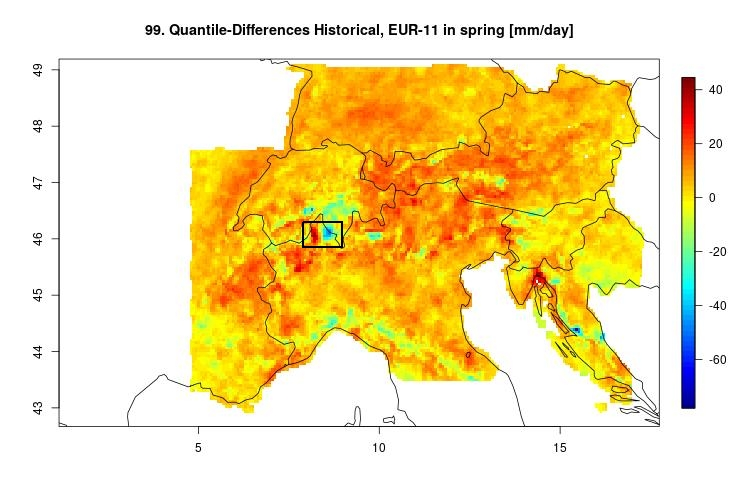
\includegraphics[width=\textwidth]{quantile_season/hist_eur11_spring.jpg}
		\caption{Historical, EUR-11 Frühling}
		\label{fig:seasons_dif:hist_eur11}
	\end{subfigure}
	\begin{subfigure}{0.49\textwidth}
		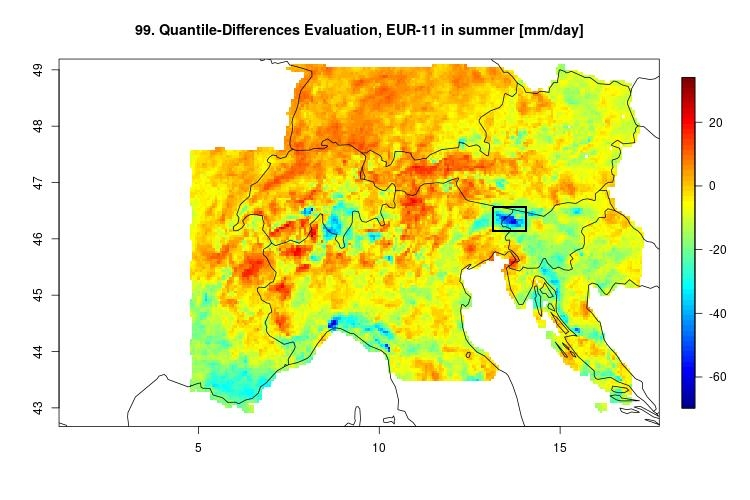
\includegraphics[width=\textwidth]{quantile_season/eval_eur11_summer.jpg}
		\caption{Evaluation, EUR-11, Sommer}
		\label{fig:seasons_dif:eval_eur_11}
	\end{subfigure}
	\begin{subfigure}{0.49\textwidth}
		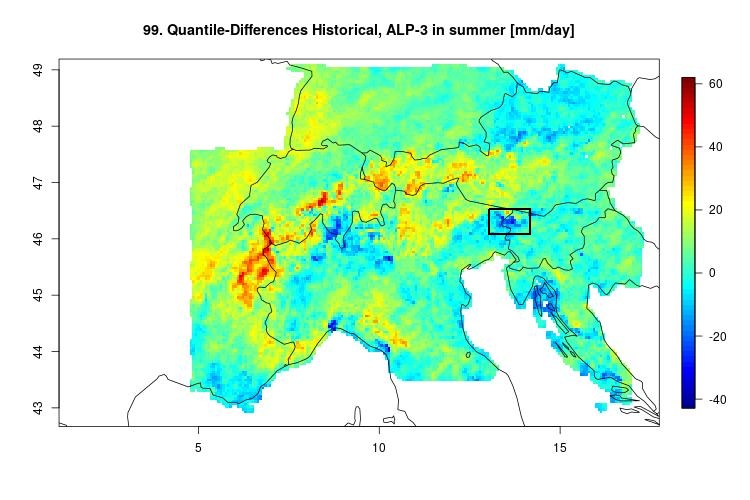
\includegraphics[width=\textwidth]{quantile_season/hist_alp3_summer.jpg}
		\caption{Historical, ALP-3 Sommer}
		\label{fig:seasons_dif:hist_alp3}
	\end{subfigure}
	\begin{subfigure}{0.49\textwidth}
		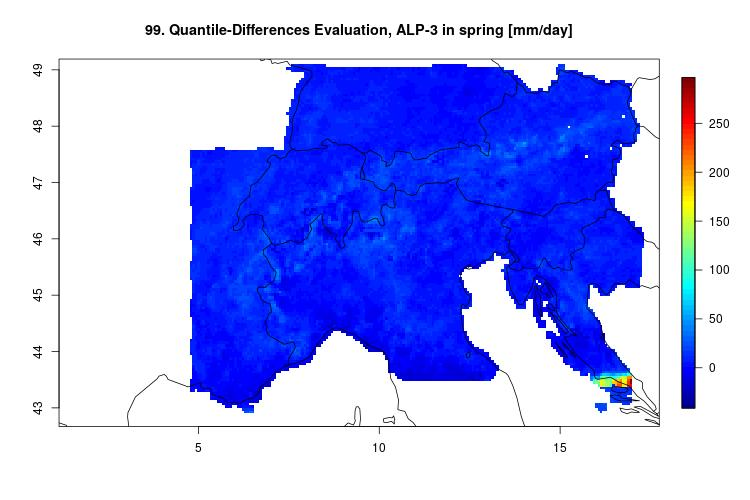
\includegraphics[width=\textwidth]{quantile_season/eval_alp3_spring.jpg}
		\caption{Evaluation, ALP-3 Frühling}
	\end{subfigure}
	\caption{Differenzen der in der Tabelle \ref{tab:season_dataset} angeführten Testfälle mit gekennzeichneten Bereichen}
	\label{fig:seasons_dif}
\end{figure}
\section{Nähere Betrachtungen der einzelnen Datensätze}
\subsection{Historical EUR-11}
Wie man in der Abbildung \ref{fig:seasons_dif:hist_eur11} erkennen kann, liegen in dem gekennzeichneten Bereichen die maximalen negativen Abweichungen direkt neben denen der maximal Positiven. Dieses Phänomen scheint mehrmals auf der Karte aufzutauchen (z.B im Bereich von Krk und im Bereich der Alpi Orobie). Dies lässt darauf schließen, dass das Modell eine große Regenzelle aufgrund von Fehlberechnungen in örtlich Fehlerhaft abbildete. Diese Vermutung kann gut durch die in Abb. \ref{fig:seasons_hist} dargestellten Niederschlagskarten nachvollzogen werden. Jedoch ist Bemerkenswert, dass das Modell solch starke Abweichungen aus dem Normalzustand überhaupt abbildet: Die Peaks, die diese Abweichungen ausmachen liegen weit über dem Durchschnitt dieser Regionen vgl. dazu Abb.\ref{fig:season:over_apgd} \& \ref{fig:season:under_apgd}\\
Um dieses Phänomen näher zu erkunden wurden der gekennzeichneten Bereich in einen Überschätzenden und einen Unterschätzenden Bereich geteilt. Die Modelldaten wurden dann im Frühling über die Fläche gemittelt und in Abb.\ref{fig:season:over_hist} \& \ref{fig:season:under_hist} gegen die Zeit aufgetragen. Dieselben Berechnungen im selben Bereich wurden für die Beobachtungsdaten vollzogen. Diese Ergebnisse wurden in der Abb.\ref{fig:season:under_apgd} \& \ref{fig:season:over_apgd} visualisiert.\\
\begin{figure}
	\begin{subfigure}{0.49\textwidth}
		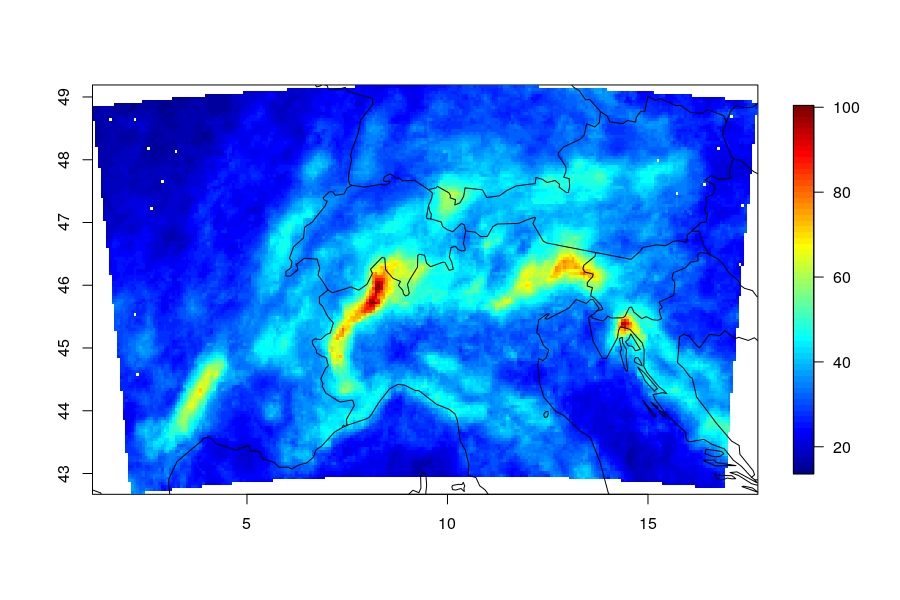
\includegraphics[width=\textwidth]{quantile_season/hist_eur_11_clean.jpg}
		\caption{Historical, EUR-11}
		\label{fig:seasons_hist:hist}
	\end{subfigure}
	\begin{subfigure}{0.49\textwidth}
		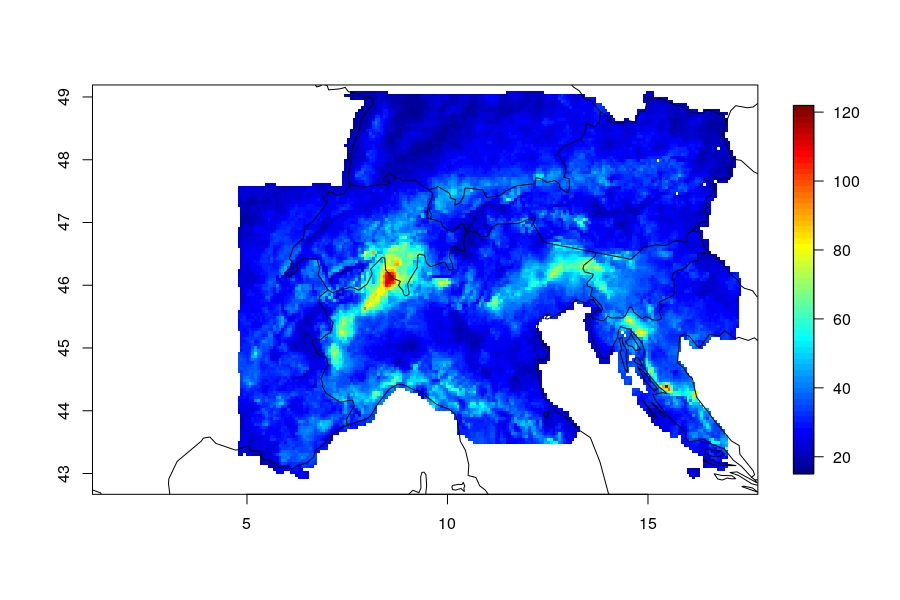
\includegraphics[width=\textwidth]{quantile_season/apgd_spring.jpg}
		\caption{APGD}
		\label{fig:seasons_hist:apgd}
	\end{subfigure}
	\caption{Die 99. Quantile der Datensätze EUR-11 und APGD für den Frühling}
	\label{fig:seasons_hist}
\end{figure}
\begin{figure}
		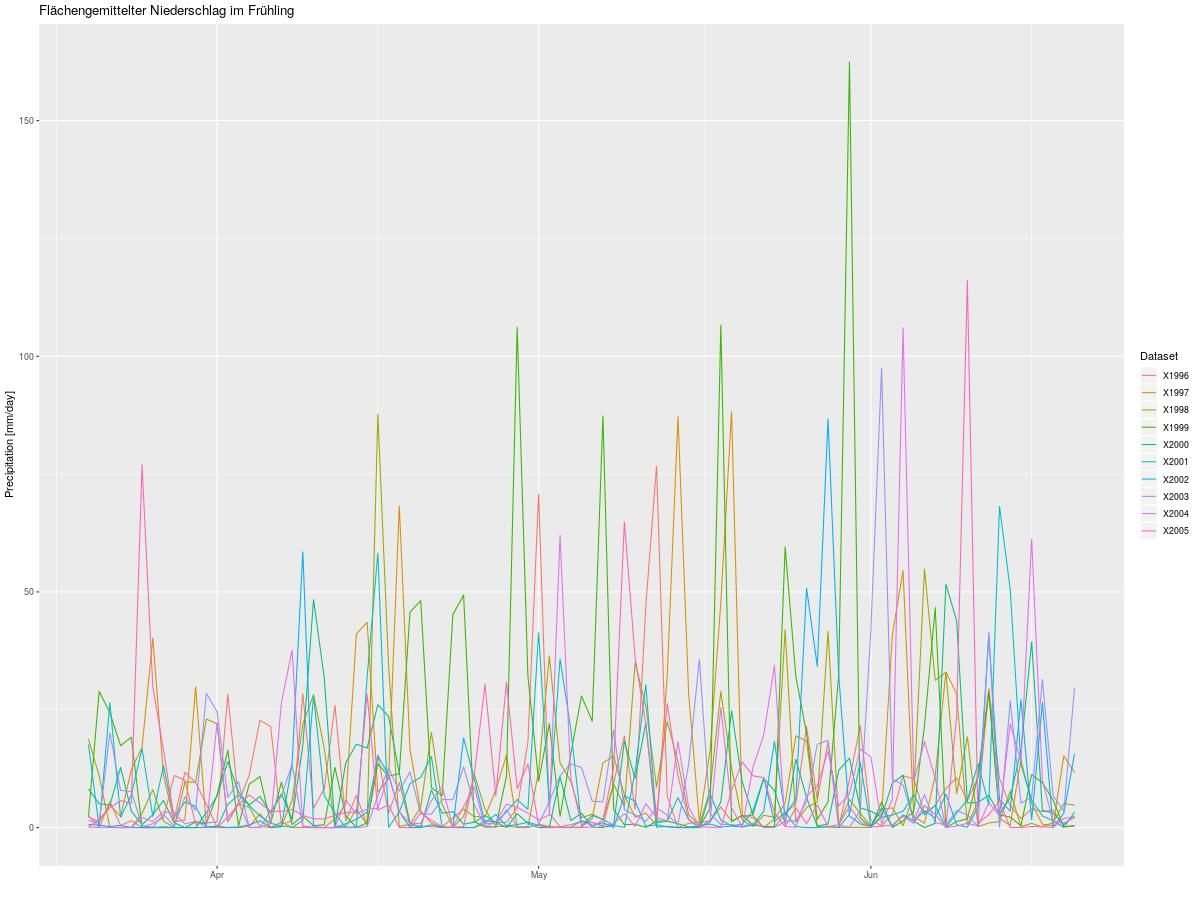
\includegraphics[width=0.95\textwidth]{quantile_season/hist_eur11_oversim1.jpg}
		\caption{Gemittelte Niederschlagsmenge im überschätzenden Bereich (vgl. Abb \ref{fig:seasons_dif:hist_eur11}) des Datensatzes Historical, EUR-11}
		\label{fig:season:over_hist}
\end{figure}
\begin{figure}
	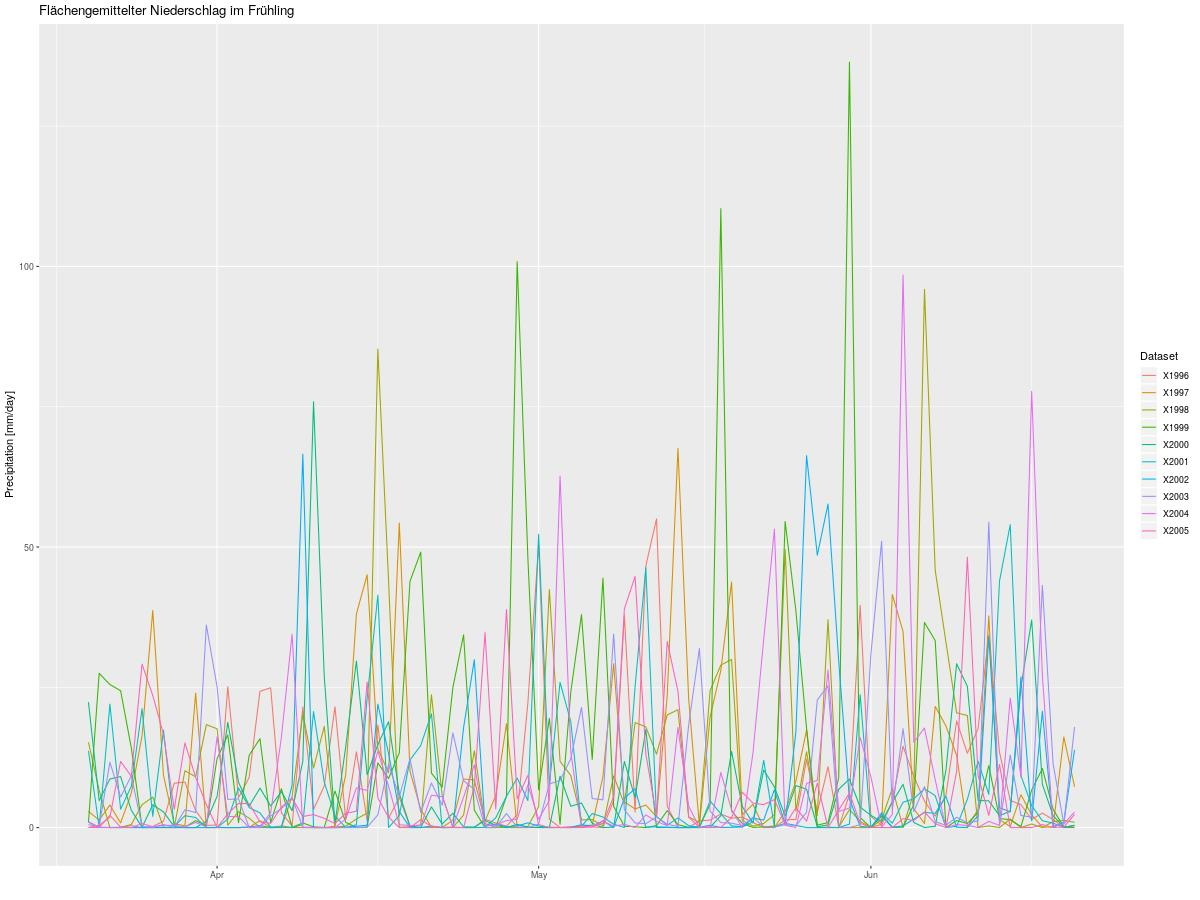
\includegraphics[width=0.95\textwidth]{quantile_season/hist_eur11_undersim1.jpg}
	\caption{Gemittelte Niederschlagsmenge im unterschätzenden Bereich (vgl. Abb \ref{fig:seasons_dif:hist_eur11}) des Datensatzes Historical, EUR-11}
	\label{fig:season:under_hist}
\end{figure}
\begin{figure}
		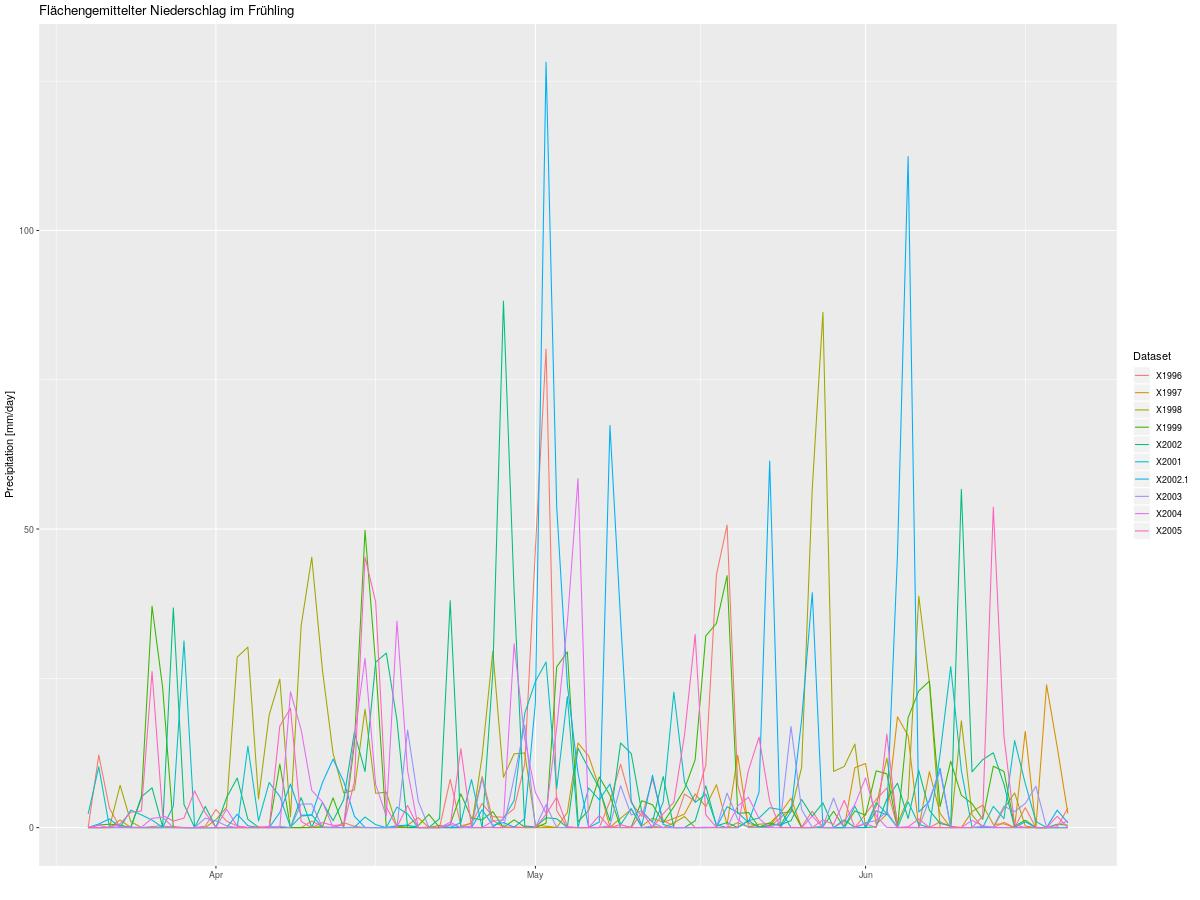
\includegraphics[width=0.95\textwidth]{quantile_season/apgd_oversim1.jpg}
		\caption{Gemittelte Niederschlagsmenge im überschätzenden Bereich (vgl. Abb \ref{fig:seasons_dif:hist_eur11}) der Beobachtungsdaten APGD}
		\label{fig:season:over_apgd}
\end{figure}
\begin{figure}
		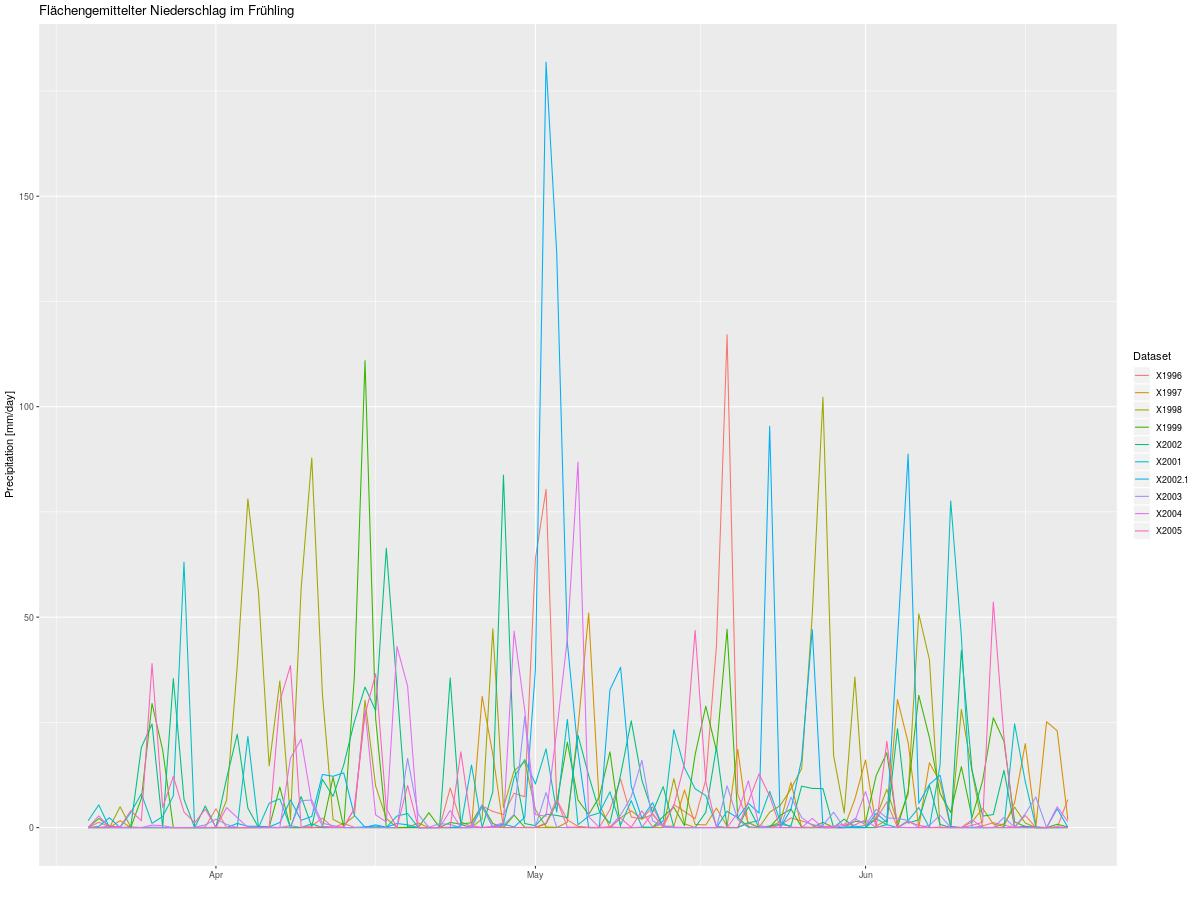
\includegraphics[width=0.95\textwidth]{quantile_season/apgd_undersim1.jpg}
		\caption{Gemittelte Niederschlagsmenge im unterschätzenden Bereich (vgl. Abb \ref{fig:seasons_dif:hist_eur11}) der Beobachtungsdaten APGD}
	\label{fig:season:under_apgd}
\end{figure}\newpage
Man erkennt gut, dass sich die Vermutungen bestätigt haben, im überschätzendem Bereich Abb.\ref{fig:season:over_hist} bildet das Modell die nahezu gleich Kurve aus wie die Beobachtungsdaten im Unterschätzendem:\ref{fig:season:under_apgd}. Dasselbe gilt für den unterschätzenden Bereich: Der Kurvenverlauf des Modells (EUR-11) gleicht der Kurve der Beobachtungsdaten im überschätzendem Bereich. Auch Beachtenswert ist, dass der entscheidende Peak vom Modell in einem anderen Monat und einem anderen Jahr vorhergesagt wird.\\

\subsection{Evaluation EUR-11}\label{sec:eval_eur_11}
In diesem Datensatz fällt auf, dass mehrere große Bereiche vom Modell unterschätzt wurden. Dies zeigt sich besonders gut in den ausgeprägten blauen Flecken der Abb.\ref{fig:seasons_dif:eval_eur_11}. Es treten kaum so starke Überschätzungen wie beim Historical Datensatz auf. Dies könnte auch an der betrachteten Jahreszeit liegen: Sommer ist die Heimat der Hitzegewitter und somit auch der kurzzeitigen Extremniederschläge, welche eine große Herausforderung in der Simulation sind. Besonders wenn die Konvektion parametrisiert wurde, wie es in diesem Modell der Fall ist. Aufgrund der Jahreszeit wird für diesen Datensatz die Temperatur und der Niederschlag in dem gekennzeichneten Bereich mit den Beobachtungsdaten verglichen.\\
Wie man in der Abbildung \ref{fig:season:under_eval_eur11} erkennt, ist der Niederschlag wieder eine für parametrisierte Konvektion typische Fluktuation nahezu gleichmäßig über die Zeit verteilt. Es gibt keine großen Ausreißer. Dies fällt besonders auf, wenn man das Mittel der Beobachtungsdaten damit vergleicht (Abb.\ref{fig:season:under_apgd_eur11}. Des Weiteren kann man der Grafik der Beobachtungsdaten entnehmen, dass sich der ausschlaggebende Peak im September 1998 befindet, da in diesem Gebiet eine Differenz von ungefähr $-60\frac{mm}{Tag}$ herrscht. Der Niederschlag in diesem Jahr schien besonders heftig auszufallen. Um nun die Temperatur in Verbindung mit der starken Abweichung im Niederschlag zu bringen, und um eventuell auch ein untypisches Wetterverhalten in diesem Jahr auszumachen. Wurde die Temperaturkarte für dieses Gebiet ausgeschnitten und, dem Niederschlag gleich, über die Fläche gemittelt.\\
Der Niederschlag wurde im betreffenden Jahr 1998 betrachtet, und es konnte zwar ein ähnliches Verhalten der Kurven beobachtet werden, jedoch mit weit zu wenig Ausschlag, wie in der Abbildung \ref{fig:seasons:undersim_eval_eur11} zu sehen ist:\\
\begin{itemize}
	\item Der Niederschlag liegt im Monat September zwar über dem Durchschnittsniederschlag, jedoch ist der Ausschlag des tatsächlich gemessene Phänomen um $100\frac{mm}{Tag}$ höher als der des Modells. Beachtenswert dabei ist zudem, dass der Niederschlag im Modell über die ganze Zeitspanne viel weniger fluktuierend vom Mittelwert abweicht als die Beobachtungsdaten dies tun.
	\item Die betreffende Temperaturkurve ist viel weniger stark ausgeprägt, jedoch ist zu erkennen, dass im Monat September, wo das Starkregenereignis auftrat die Modelldaten eine auf den Durchschnitt bezogene kältere Temperatur vorhersagte als in den Beobachtungsdaten gemessen wurde. Zudem ist beachtenswert, dass die Ausschläge über die ganze Zeitspanne oft gegenläufig sind.
\end{itemize}

\begin{figure}
	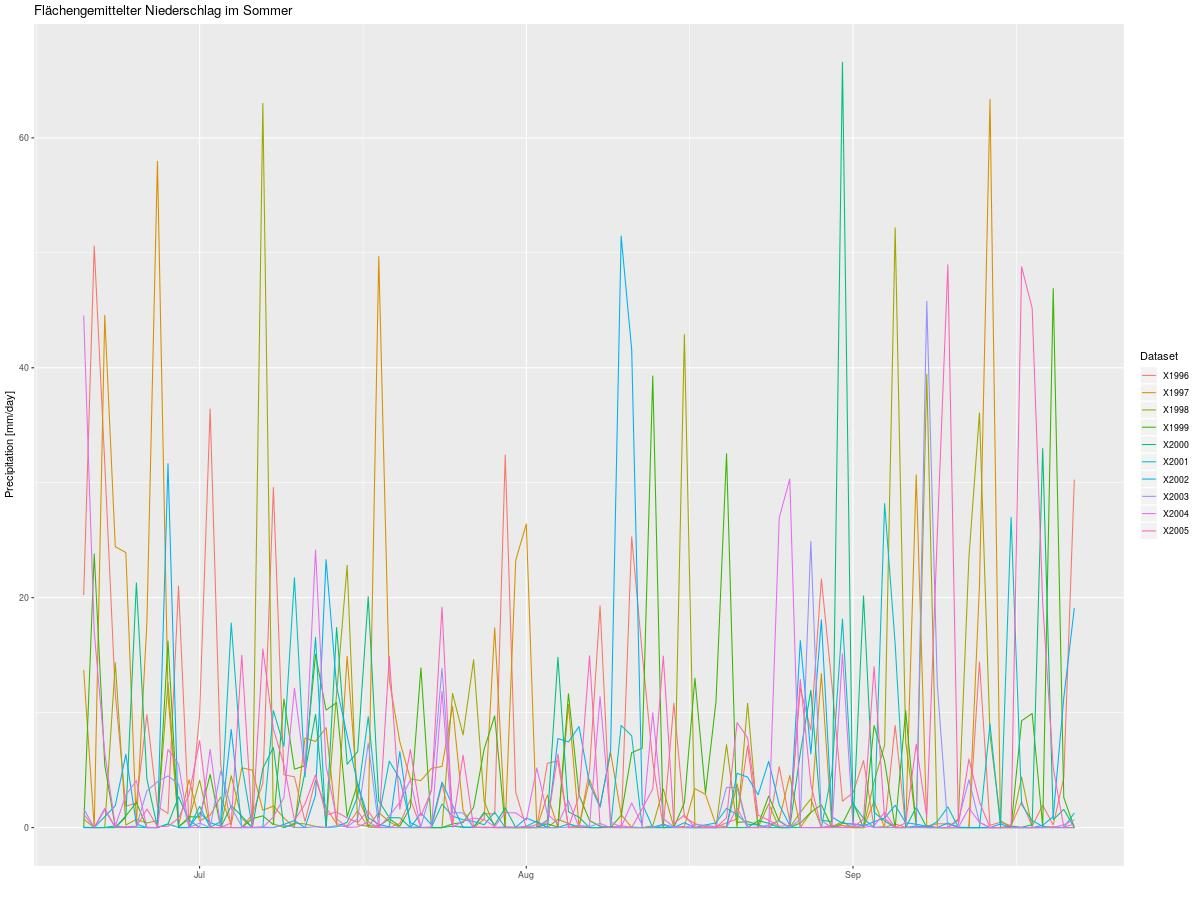
\includegraphics[width=0.95\textwidth]{quantile_season/eval_eur11_undersim.jpg}
	\caption{Flächenmittel des Niederschlags im unterschätzenden Gebiet, gekennzeichnet in Abb.\ref{fig:seasons_dif:hist_eur11} für den Datensatz Evaluation, EUR-11}
	\label{fig:season:under_eval_eur11}
\end{figure}
\begin{figure}
	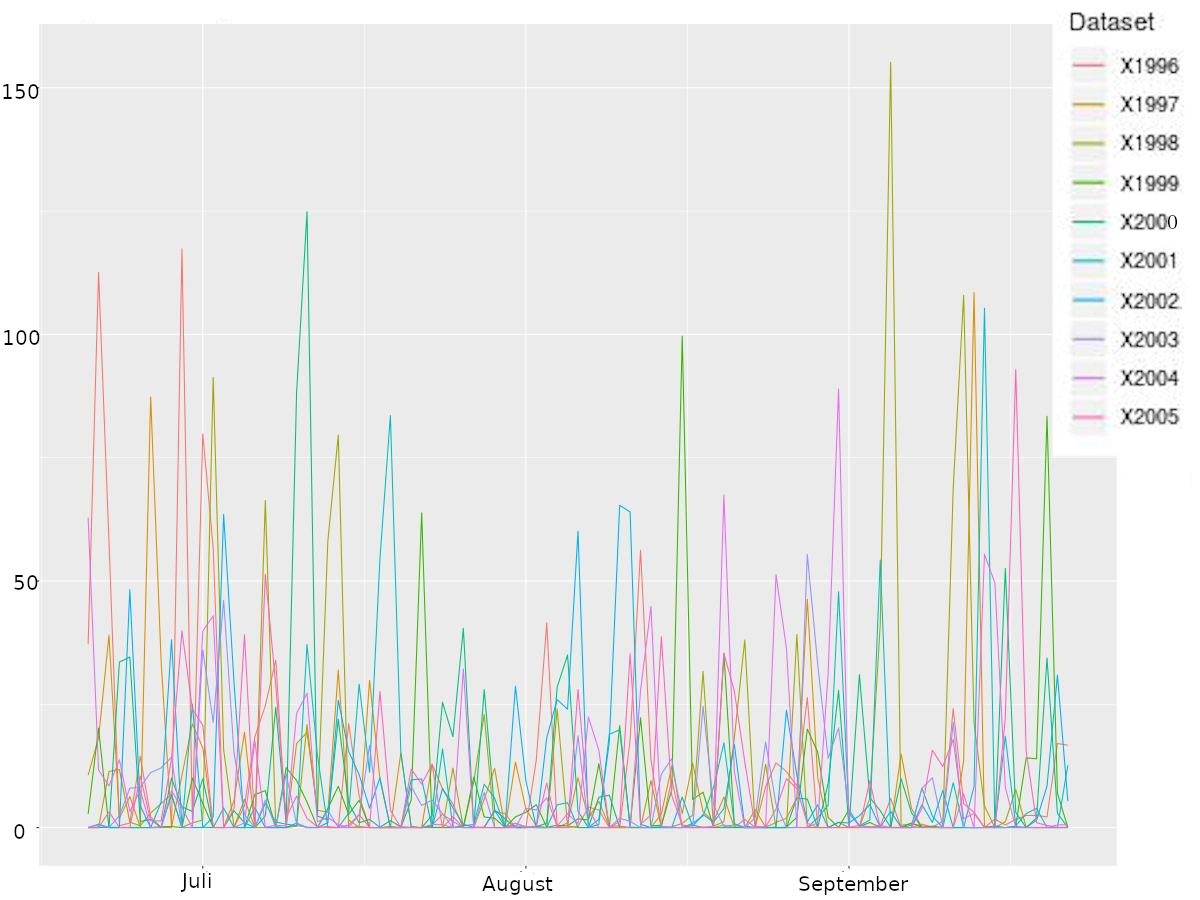
\includegraphics[width=0.95\textwidth]{quantile_season/apgd_undersim_eur11.jpg}
	\caption{Flächenmittel des Niederschlags im unterschätzenden Gebiet, gekennzeichnet in Abb.\ref{fig:seasons_dif:hist_eur11} für den Beobachtungs-Datensatz APGD}
	\label{fig:season:under_apgd_eur11}
\end{figure}
\begin{figure}
	\begin{subfigure}{0.49\textwidth}
		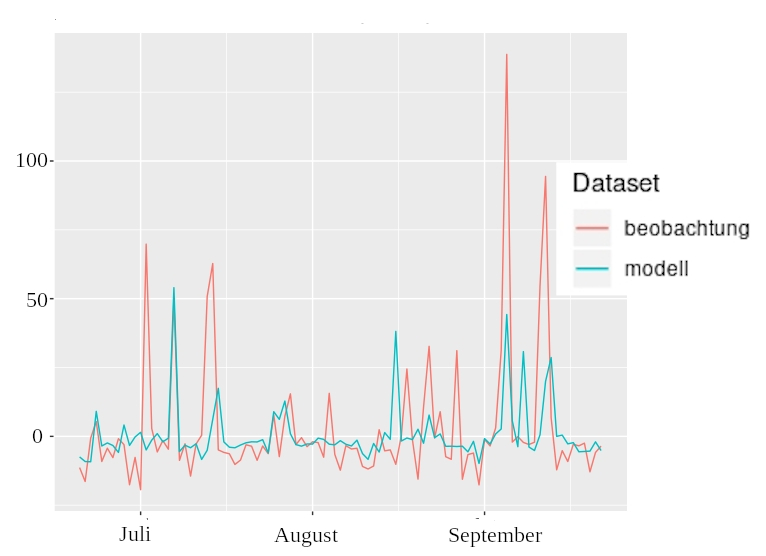
\includegraphics[width=\textwidth]{quantile_season/middle_pr_undersim_eur11.jpg}
		\caption{Die Differenzen der Modelldaten(Eval-EUR-11) und der Beobachtungsdaten vom mittlerem Niederschlag in der in Abb.\ref{fig:seasons_dif:eval_eur_11} gekennzeichneten Fläche (im Jahr 1998)}
	\end{subfigure}
	\begin{subfigure}{0.49\textwidth}
		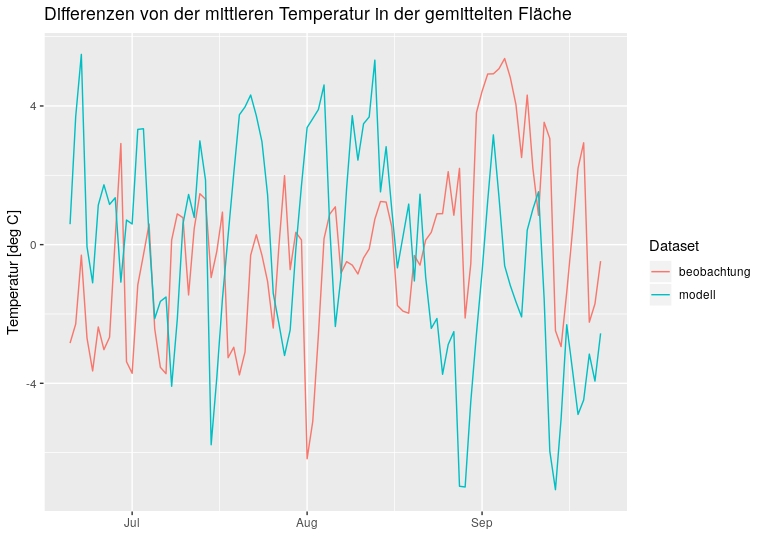
\includegraphics[width=\textwidth]{quantile_season/middle_temp_undersim_eur11.jpg}
		\caption{Die Differenzen der Modelldaten (Eval-EUR-11) und der Beobachtungsdaten von den mittleren Temperaturen in der in Abb.\ref{fig:seasons_dif:eval_eur_11} gekennzeichneten Fläche (im Jahr 1998)}
	\end{subfigure}
	\caption{Differenz der Temperatur und des Niederschlags zum Durchschnitt}
	\label{fig:seasons:undersim_eval_eur11}
\end{figure}\newpage
\subsection{Historical ALP-3}
Wie in der Abbildung \ref{fig:seasons_dif:hist_alp3} zu sehen ist, wird in diesem Kapitel derselbe Bereich evaluiert, wie bereits im zuvor im Kapitel \ref{sec:eval_eur_11}. Dadurch können die beiden Modelle und auch die Antriebsdaten gegeneinander verglichen werden. Da das Modell CCLM5-0-9 im ALP-3 Historical Datensatz mit historischen Daten des globalen Klimamodells MPI-ESM-LR angetrieben, dadurch sollten theoretisch größere Abweichungen herrschen als in dem mit Re-Analysedaten betriebenen, wenn auch gröber aufgelösten Evaluation, EUR11.\\
Wieder wurden wie im Kapitel zuvor schon die Daten über die in Abb.\ref{fig:seasons_dif:hist_alp3} gekennzeichnete Fläche gemittelt und mit den Beobachtungsdaten verglichen, da in dem selben Bereich eine relativ große negative Abweichung vorzufinden war. Dabei blieb natürlich der Beobachtungsdatensatz derselbe und es wird deshalb darauf verzichtet, den Plot in Abb.\ref{fig:season:under_apgd_eur11} nochmal abzubilden. Die Modelldaten sind in der Abb.\ref{fig:season:under_hist_alp3}\\
Man erkennt, dass sich das Muster für den Niederschlag kaum verändert hat. Der Zusammenhang mit den Beobachtungsdaten hat sich sogar etwas verschlechtert: Da die Übereinstimmung des Peaks im September überhaupt nicht mehr gegeben ist. Auch beim Betrachten der Abb.\ref{fig:season:under_hist_alp3} fällt dies bereits auf.\\
Die Temperatur scheint jedoch um einiges besser den Gegebenheiten zu entsprechen, die Fluktuationen über und unter der Durchschnittstemperatur entsprechen nahezu perfekt denen in den Beobachtungsdaten. Nur wiederum im September scheint ein größerer Fehler berechnet worden zu sein. Somit kann für das Konvektion-Erlaubende Klimamodell gesagt werden, dass die Temperaturfluktuationen im Sommer um einiges besser dargestellt werden.
\begin{figure}[h]
	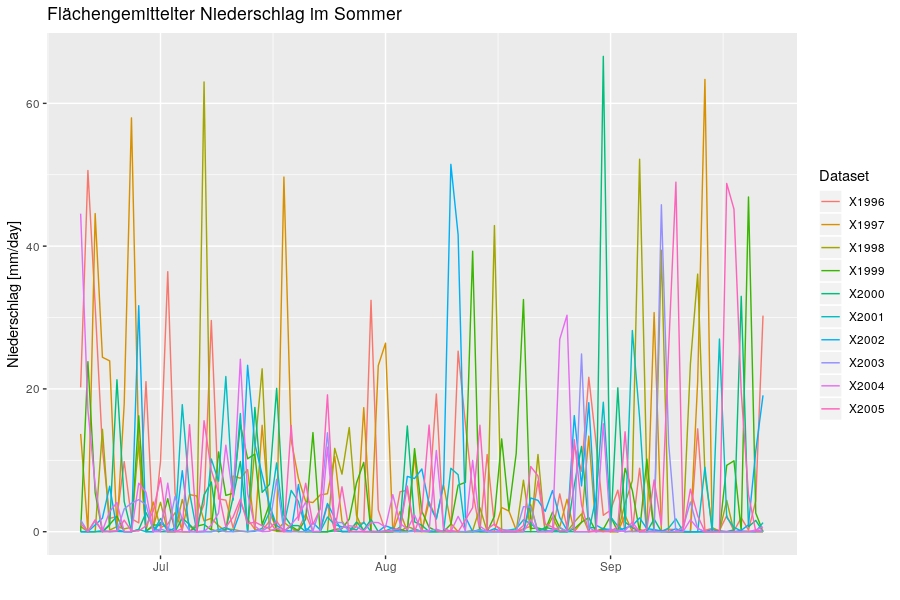
\includegraphics[width=\textwidth]{quantile_season/hist_alp3_undersim.jpg}
	\caption{Niederschlagsverlauf im Datensatz Historical, ALP-3 für den in Abb.\ref{fig:seasons_dif:hist_alp3} gekennzeichneten Bereich, gemittelt über dessen Fläche}
	\label{fig:season:under_hist_alp3}
\end{figure}
\begin{figure}
	\begin{subfigure}{0.49\textwidth}
		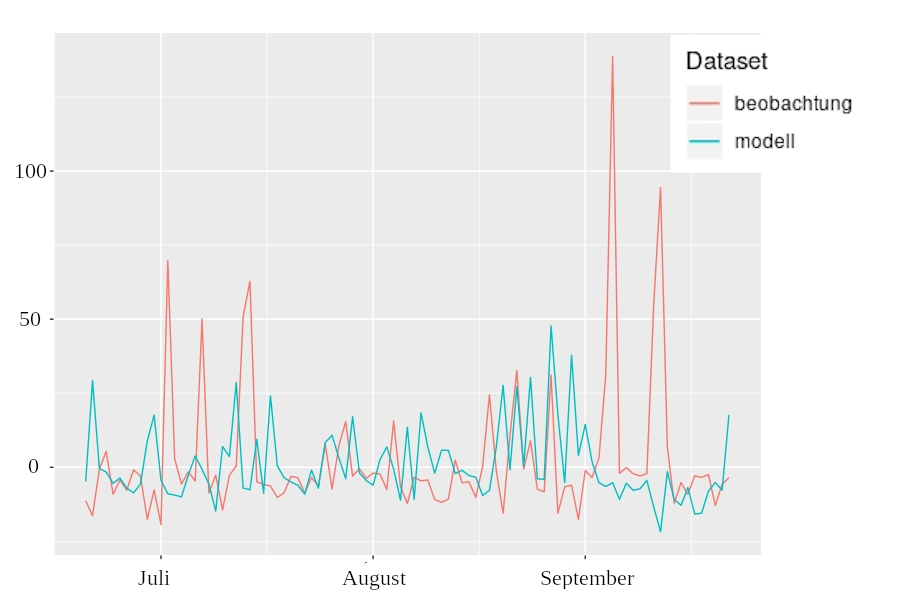
\includegraphics[width=\textwidth]{quantile_season/dif_pr_undersim_alp3.jpeg}
		\caption{Die Differenzen der Modelldaten(Historical - ALP-3) und der Beobachtungsdaten vom mittlerem Niederschlag in der in Abb.\ref{fig:seasons_dif:hist_alp3} gekennzeichneten Fläche (im Jahr 1998)}
	\end{subfigure}
	\begin{subfigure}{0.49\textwidth}
		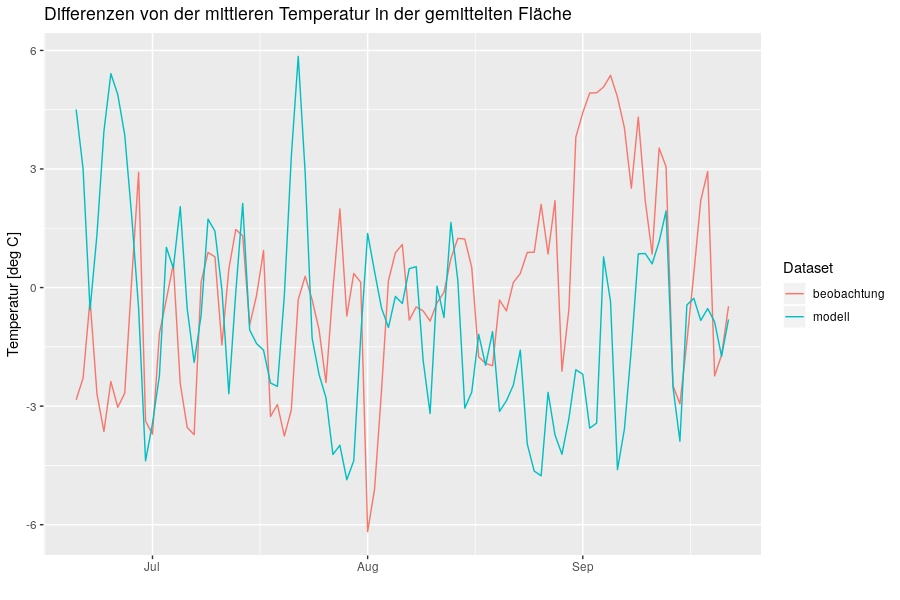
\includegraphics[width=\textwidth]{quantile_season/dif_temp_undersim_alp3.jpeg}
		\caption{Die Differenzen der Modelldaten (Historical - ALP-3) und der Beobachtungsdaten von den mittleren Temperaturen in der in Abb.\ref{fig:seasons_dif:hist_alp3} gekennzeichneten Fläche (im Jahr 1998)}
	\end{subfigure}
	\caption{Differenz der Temperatur und des Niederschlags zum entsprechenden Durchschnitt}
	\label{fig:seasons:mean_alp3}
\end{figure}
\subsection{Evaluation ALP-3}
Um diesen Datensatz und dessen größere Abweichungen darzustellen wurde zunächst der Ausreißer im Süden Kroatiens ausgeschnitten um dessen Verfälschung auszublenden. Die Karte, die sich daraus ergab findet man in der Abb.